
\section{Theorie}
\label{sec:Theorie}
Die Ausbreitungsvorgänge von Licht können gut beschrieben werden, indem angenommen
wird, dass Licht eine elektromagnetische Welle mit ist. Aus den maxwellschen Gleichungen
ergibt sich zusätzlich, dass meherere Welle durch Superposition überlagert werden können.
Jedoch ergeben sich für sichtbares Licht Frequenzen im Bereich von $\SI{10 E15}{\hertz}$,
weswegen der Zusammenhang nicht auf direktem Weg experimentell prüfbar ist. Daher
erfolgt die Superposition indirekt über die Lichtintensität $I$. Für eine Überlagerung von zwei unabhängigen Wellen gleicher Intensität ergibt sich:
\begin{equation}
  I_\text{Ges} = 2 A | E_0 |^2 \left(1 + \cos(\delta_2 - \delta_1) \right)\text{,}
\end{equation}
mit der Summe der Einzelintensitäten $2 A | E_0 |^2$ und einem Interferenzterm. Letzterer
ist abhängig von der Phasenverschiebung beider Welle und kann die Gesamtintensität entweder verstärken oder bis zur Auslöschung reduzieren.
Auf einem Schirm zeigt sich das entstehende Interferenzbild in Form von dunklen und hellen Streifen.

Es zeigt sich jedoch, dass bei der Überlagerung von Lichtstrahlen aus unabhängigen
Lichtquellen im Regelfall keine Interferenz zu erkennen ist. Der Grund hierfür liegt
 in den unterschiedlichen Phasenkonstanten, welche bei normalen Leuchtmitteln aufgrund
 der quantenmechanischen Natur der Lichtemission durch Elektronen statistisch verteilt sind.
 Solches Licht wird als inkohärent bezeichnet. Daher wird ein Laser verwendet, bei welchem die Lichtemission gleich getaktet ist.
 Eine weitere Möglichkeit Interferenzeffekte beobachten zu können liegt darin, dass Licht einer Quelle zu teilen und.
 Die entstandenen Lichtstrahlen sind natürlich gleich getaktet und erzeugen bei einer erneuten Zusammenführung
 daher ein erkennbares Interferenzbild. Für die Gangunterschiede zu Erzeugung von Interferenzmaxima und Minima gilt:
 \begin{equation}
   \Delta_\text{max} = n \lambda
 \end{equation}
   \begin{equation}
   \Delta_\text{min} = \left(2 n+1\right)\frac{\lambda}{2}
 \end{equation}
Es ist jedoch darauf zu achten das die Gangunterschiede nicht deutlich größer als
die Wellenlänge ausfällt, da die Elektronen nur endliche Wellenzüge emittiert. Fallen
die Gangunterschiede nun zu groß aus, treffen Lichtstrahlen aus unterschiedlichen Emissionen
 zusammen und sind daher nicht mehr kohärent. Für den maximal möglichen Gangunterschied gilt:
 \begin{equation}
   l = N \lambda \text{,}
 \end{equation}
mit der maximal auf dem Schirm beobachtbaren Maximumanzahl $N$. Wird eine punktförmige
Lichtquelle angenommen, ist eine Intensitätsverteilung für eine Lichtwelle der Winkelgeschwindigkeit $\omega$ gegeben durch:
\begin{equation}
  I(\omega) = 4 E^2_0 \frac{\sin(\omega -\omega_0) l }{\left(\omega - \omega_0\right)^2 2 c}\text{.}
  \end{equation}
  In der Praxis liegen jedoch Lichtquellen mit endlicher Ausbreitung vor. Daher kommt es bei
  Betrachtung eines festen Punktes auf dem Schirm wieder zu einer Überlagerung von Wellen
  mit einem kontinuierlichem Spektrum von Gangunterschieden und einem resultierenden Verschwinden des Interferenzbildes.
  Der Effekt kann nicht aufgehoben werden, ist jedoch reduzierbar. Hierzu müssen entweder die Abmessungen der Lichtquelle
  oder der beobachtete Winkelbereich klein gehalten werden.

  \subsection{Das Michelson-Interferometer}


  \begin{figure}
  	\centering
  	\caption{Der prinzipielle Aufbau des Michelson-Interferometer \cite{V401}.}
  	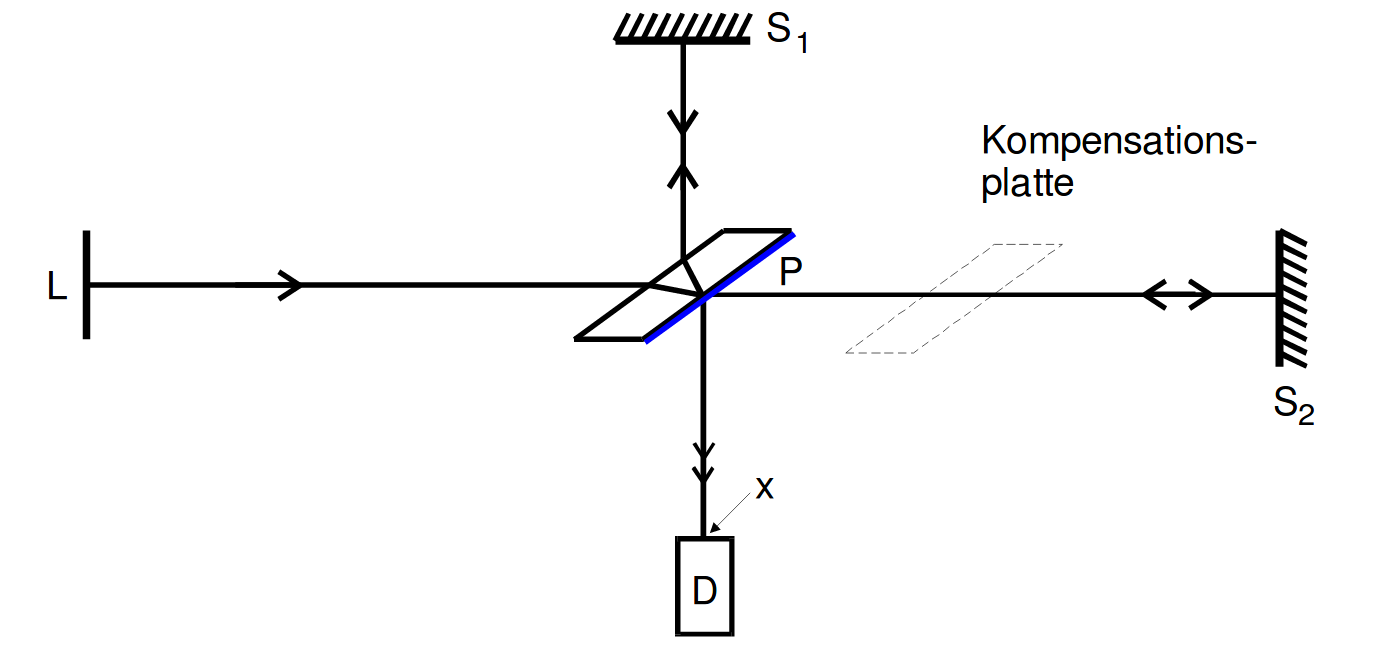
\includegraphics[width=\linewidth-150pt,height=\textheight-150pt,keepaspectratio]{content/theoriebau.png}
  	\label{fig:aufbauth}
  \end{figure}
  Für das Michelson-Interferometer werden nun beide Effekte kombiniert. Ein Laser trifft
  auf einen halbdurchlässigen Spiegel, welcher im $\SI{45}{\degree}$ aufgestellt ist und
  den Strahl in zwei zueinander kohärente Teilstrahlen aufspaltet. Beide Strahlen gelangen anschließend
  gemäß Abb. \ref{fig:aufbauth} jeweils auf einen Spiegel und werden wieder zurückgeworfen. Beim
  Halbdurchlässigen Spiegel kommen beide wieder zur Interferenz und werden wieder zum Teil auf
  einen Detektor reflektiert. Wird nun der obere Spiegel weiter nach oben verschoben,
  ändert sich der Gangunterschied und damit auch das Interferenzbild. Aus der Verschiebungsstrecke
  $\Delta d$ sowie in der Strecke auftretenden Maximaanzahl $z$ lässt sich die Wellenlänge der Lichtquelle durch:
  \begin{equation}
    \lambda = \frac{2 \Delta d}{z}\label{lambda}
    \end{equation}
    bestimmen. Auf ganz ähnliche Weise kann auch eine Veränderung der optischen Wegstrecke
     auch durch Veänderung $\Delta n$ des Brechungsindexes erfolgen. In diesem Fall wird eine teilweise evakuierte Messzelle verwendet.
     Die Effekte der Box an sich können durch eine Kompensationsplatte ausgeglichen werden. Für die Wellenlänge gilt dann:
     \begin{equation}
       \lambda = \frac{2 b \Delta n }{z}\text{.}\label{nausdeltan}
       \end{equation}
Da beim Michelson-Interferometer normalerweise mit divergenten Lichtsrahlen gearbeitet wird,
bilden die Interferenzmaxima und Minima Ringe, welche entweder aus dem Zentrum entstehen oder in ihm verschwinden.
